% Options for packages loaded elsewhere
\PassOptionsToPackage{unicode}{hyperref}
\PassOptionsToPackage{hyphens}{url}
\PassOptionsToPackage{dvipsnames,svgnames,x11names}{xcolor}
%
\documentclass[
  letterpaper,
  DIV=11,
  numbers=noendperiod]{scrreprt}

\usepackage{amsmath,amssymb}
\usepackage{lmodern}
\usepackage{iftex}
\ifPDFTeX
  \usepackage[T1]{fontenc}
  \usepackage[utf8]{inputenc}
  \usepackage{textcomp} % provide euro and other symbols
\else % if luatex or xetex
  \usepackage{unicode-math}
  \defaultfontfeatures{Scale=MatchLowercase}
  \defaultfontfeatures[\rmfamily]{Ligatures=TeX,Scale=1}
\fi
% Use upquote if available, for straight quotes in verbatim environments
\IfFileExists{upquote.sty}{\usepackage{upquote}}{}
\IfFileExists{microtype.sty}{% use microtype if available
  \usepackage[]{microtype}
  \UseMicrotypeSet[protrusion]{basicmath} % disable protrusion for tt fonts
}{}
\makeatletter
\@ifundefined{KOMAClassName}{% if non-KOMA class
  \IfFileExists{parskip.sty}{%
    \usepackage{parskip}
  }{% else
    \setlength{\parindent}{0pt}
    \setlength{\parskip}{6pt plus 2pt minus 1pt}}
}{% if KOMA class
  \KOMAoptions{parskip=half}}
\makeatother
\usepackage{xcolor}
\setlength{\emergencystretch}{3em} % prevent overfull lines
\setcounter{secnumdepth}{5}
% Make \paragraph and \subparagraph free-standing
\ifx\paragraph\undefined\else
  \let\oldparagraph\paragraph
  \renewcommand{\paragraph}[1]{\oldparagraph{#1}\mbox{}}
\fi
\ifx\subparagraph\undefined\else
  \let\oldsubparagraph\subparagraph
  \renewcommand{\subparagraph}[1]{\oldsubparagraph{#1}\mbox{}}
\fi

\usepackage{color}
\usepackage{fancyvrb}
\newcommand{\VerbBar}{|}
\newcommand{\VERB}{\Verb[commandchars=\\\{\}]}
\DefineVerbatimEnvironment{Highlighting}{Verbatim}{commandchars=\\\{\}}
% Add ',fontsize=\small' for more characters per line
\usepackage{framed}
\definecolor{shadecolor}{RGB}{241,243,245}
\newenvironment{Shaded}{\begin{snugshade}}{\end{snugshade}}
\newcommand{\AlertTok}[1]{\textcolor[rgb]{0.68,0.00,0.00}{#1}}
\newcommand{\AnnotationTok}[1]{\textcolor[rgb]{0.37,0.37,0.37}{#1}}
\newcommand{\AttributeTok}[1]{\textcolor[rgb]{0.40,0.45,0.13}{#1}}
\newcommand{\BaseNTok}[1]{\textcolor[rgb]{0.68,0.00,0.00}{#1}}
\newcommand{\BuiltInTok}[1]{\textcolor[rgb]{0.00,0.23,0.31}{#1}}
\newcommand{\CharTok}[1]{\textcolor[rgb]{0.13,0.47,0.30}{#1}}
\newcommand{\CommentTok}[1]{\textcolor[rgb]{0.37,0.37,0.37}{#1}}
\newcommand{\CommentVarTok}[1]{\textcolor[rgb]{0.37,0.37,0.37}{\textit{#1}}}
\newcommand{\ConstantTok}[1]{\textcolor[rgb]{0.56,0.35,0.01}{#1}}
\newcommand{\ControlFlowTok}[1]{\textcolor[rgb]{0.00,0.23,0.31}{#1}}
\newcommand{\DataTypeTok}[1]{\textcolor[rgb]{0.68,0.00,0.00}{#1}}
\newcommand{\DecValTok}[1]{\textcolor[rgb]{0.68,0.00,0.00}{#1}}
\newcommand{\DocumentationTok}[1]{\textcolor[rgb]{0.37,0.37,0.37}{\textit{#1}}}
\newcommand{\ErrorTok}[1]{\textcolor[rgb]{0.68,0.00,0.00}{#1}}
\newcommand{\ExtensionTok}[1]{\textcolor[rgb]{0.00,0.23,0.31}{#1}}
\newcommand{\FloatTok}[1]{\textcolor[rgb]{0.68,0.00,0.00}{#1}}
\newcommand{\FunctionTok}[1]{\textcolor[rgb]{0.28,0.35,0.67}{#1}}
\newcommand{\ImportTok}[1]{\textcolor[rgb]{0.00,0.46,0.62}{#1}}
\newcommand{\InformationTok}[1]{\textcolor[rgb]{0.37,0.37,0.37}{#1}}
\newcommand{\KeywordTok}[1]{\textcolor[rgb]{0.00,0.23,0.31}{#1}}
\newcommand{\NormalTok}[1]{\textcolor[rgb]{0.00,0.23,0.31}{#1}}
\newcommand{\OperatorTok}[1]{\textcolor[rgb]{0.37,0.37,0.37}{#1}}
\newcommand{\OtherTok}[1]{\textcolor[rgb]{0.00,0.23,0.31}{#1}}
\newcommand{\PreprocessorTok}[1]{\textcolor[rgb]{0.68,0.00,0.00}{#1}}
\newcommand{\RegionMarkerTok}[1]{\textcolor[rgb]{0.00,0.23,0.31}{#1}}
\newcommand{\SpecialCharTok}[1]{\textcolor[rgb]{0.37,0.37,0.37}{#1}}
\newcommand{\SpecialStringTok}[1]{\textcolor[rgb]{0.13,0.47,0.30}{#1}}
\newcommand{\StringTok}[1]{\textcolor[rgb]{0.13,0.47,0.30}{#1}}
\newcommand{\VariableTok}[1]{\textcolor[rgb]{0.07,0.07,0.07}{#1}}
\newcommand{\VerbatimStringTok}[1]{\textcolor[rgb]{0.13,0.47,0.30}{#1}}
\newcommand{\WarningTok}[1]{\textcolor[rgb]{0.37,0.37,0.37}{\textit{#1}}}

\providecommand{\tightlist}{%
  \setlength{\itemsep}{0pt}\setlength{\parskip}{0pt}}\usepackage{longtable,booktabs,array}
\usepackage{calc} % for calculating minipage widths
% Correct order of tables after \paragraph or \subparagraph
\usepackage{etoolbox}
\makeatletter
\patchcmd\longtable{\par}{\if@noskipsec\mbox{}\fi\par}{}{}
\makeatother
% Allow footnotes in longtable head/foot
\IfFileExists{footnotehyper.sty}{\usepackage{footnotehyper}}{\usepackage{footnote}}
\makesavenoteenv{longtable}
\usepackage{graphicx}
\makeatletter
\def\maxwidth{\ifdim\Gin@nat@width>\linewidth\linewidth\else\Gin@nat@width\fi}
\def\maxheight{\ifdim\Gin@nat@height>\textheight\textheight\else\Gin@nat@height\fi}
\makeatother
% Scale images if necessary, so that they will not overflow the page
% margins by default, and it is still possible to overwrite the defaults
% using explicit options in \includegraphics[width, height, ...]{}
\setkeys{Gin}{width=\maxwidth,height=\maxheight,keepaspectratio}
% Set default figure placement to htbp
\makeatletter
\def\fps@figure{htbp}
\makeatother
\newlength{\cslhangindent}
\setlength{\cslhangindent}{1.5em}
\newlength{\csllabelwidth}
\setlength{\csllabelwidth}{3em}
\newlength{\cslentryspacingunit} % times entry-spacing
\setlength{\cslentryspacingunit}{\parskip}
\newenvironment{CSLReferences}[2] % #1 hanging-ident, #2 entry spacing
 {% don't indent paragraphs
  \setlength{\parindent}{0pt}
  % turn on hanging indent if param 1 is 1
  \ifodd #1
  \let\oldpar\par
  \def\par{\hangindent=\cslhangindent\oldpar}
  \fi
  % set entry spacing
  \setlength{\parskip}{#2\cslentryspacingunit}
 }%
 {}
\usepackage{calc}
\newcommand{\CSLBlock}[1]{#1\hfill\break}
\newcommand{\CSLLeftMargin}[1]{\parbox[t]{\csllabelwidth}{#1}}
\newcommand{\CSLRightInline}[1]{\parbox[t]{\linewidth - \csllabelwidth}{#1}\break}
\newcommand{\CSLIndent}[1]{\hspace{\cslhangindent}#1}

\KOMAoption{captions}{tableheading}
\makeatletter
\makeatother
\makeatletter
\@ifpackageloaded{bookmark}{}{\usepackage{bookmark}}
\makeatother
\makeatletter
\@ifpackageloaded{caption}{}{\usepackage{caption}}
\AtBeginDocument{%
\ifdefined\contentsname
  \renewcommand*\contentsname{Table of contents}
\else
  \newcommand\contentsname{Table of contents}
\fi
\ifdefined\listfigurename
  \renewcommand*\listfigurename{List of Figures}
\else
  \newcommand\listfigurename{List of Figures}
\fi
\ifdefined\listtablename
  \renewcommand*\listtablename{List of Tables}
\else
  \newcommand\listtablename{List of Tables}
\fi
\ifdefined\figurename
  \renewcommand*\figurename{Figure}
\else
  \newcommand\figurename{Figure}
\fi
\ifdefined\tablename
  \renewcommand*\tablename{Table}
\else
  \newcommand\tablename{Table}
\fi
}
\@ifpackageloaded{float}{}{\usepackage{float}}
\floatstyle{ruled}
\@ifundefined{c@chapter}{\newfloat{codelisting}{h}{lop}}{\newfloat{codelisting}{h}{lop}[chapter]}
\floatname{codelisting}{Listing}
\newcommand*\listoflistings{\listof{codelisting}{List of Listings}}
\makeatother
\makeatletter
\@ifpackageloaded{caption}{}{\usepackage{caption}}
\@ifpackageloaded{subcaption}{}{\usepackage{subcaption}}
\makeatother
\makeatletter
\@ifpackageloaded{tcolorbox}{}{\usepackage[many]{tcolorbox}}
\makeatother
\makeatletter
\@ifundefined{shadecolor}{\definecolor{shadecolor}{rgb}{.97, .97, .97}}
\makeatother
\makeatletter
\makeatother
\ifLuaTeX
  \usepackage{selnolig}  % disable illegal ligatures
\fi
\IfFileExists{bookmark.sty}{\usepackage{bookmark}}{\usepackage{hyperref}}
\IfFileExists{xurl.sty}{\usepackage{xurl}}{} % add URL line breaks if available
\urlstyle{same} % disable monospaced font for URLs
\hypersetup{
  pdftitle={Cell growth and proliferation: mathematical modeling and simulation},
  pdfauthor={César Vargas},
  colorlinks=true,
  linkcolor={blue},
  filecolor={Maroon},
  citecolor={Blue},
  urlcolor={Blue},
  pdfcreator={LaTeX via pandoc}}

\title{Cell growth and proliferation: mathematical modeling and
simulation}
\author{César Vargas}
\date{11/29/22}

\begin{document}
\maketitle
\ifdefined\Shaded\renewenvironment{Shaded}{\begin{tcolorbox}[interior hidden, boxrule=0pt, enhanced, borderline west={3pt}{0pt}{shadecolor}, frame hidden, sharp corners, breakable]}{\end{tcolorbox}}\fi

\renewcommand*\contentsname{Table of contents}
{
\hypersetup{linkcolor=}
\setcounter{tocdepth}{2}
\tableofcontents
}
\bookmarksetup{startatroot}

\hypertarget{section}{%
\chapter{}\label{section}}

\bookmarksetup{startatroot}

\hypertarget{introduction}{%
\chapter{Introduction}\label{introduction}}

\hypertarget{getting-started-in-cell-division-modeling}{%
\section{Getting started in cell division
modeling}\label{getting-started-in-cell-division-modeling}}

Let the cell size \(s\) grow exponentially according to the equation
\[\frac{ds}{dt}=\alpha s, \, s(0)=s_0,\] where \(\alpha\) is the growth
rate, \(s_0\) is the initial cell size, and \(t\) is the experiment
time. Also, let the cell cycle time \(\tau\) be the time it takes for a
cell to grow and divide. The cell cycle progress is represented by the
equation \[\frac{d\tau}{dt}=1, \, \tau(0)=0.\]

A division event occurs when a cell splits into two daughter cells. This
event resets both the cell size to half and the cell cycle time to zero,
that is, \[ s \mapsto s / 2, \quad \tau \mapsto 0,\] marking the end of
one cycle and the start of a new one. Let \(P(\tau)\) define when
division happens as per \[P(\tau)=U(\tau-\bar{\tau})=\begin{cases}
    1,  \text{ if } \tau > \bar{\tau} \\
    0,  \text{ otherwise,}
\end{cases}\] where \(U(\tau-\bar{\tau})\) is the unit step function and
\(\bar{\tau}\) is the time to division since the start of the cell
cycle. Cell performs a division event if \(P(\tau)=1\).

The division rate can be defined as \[\begin{aligned}
    p(\tau)&=\frac{d P}{d\tau}\\
    &=\delta(\tau-\bar{\tau}),
\end{aligned}\] where \(\delta(\tau)\) is the \emph{Delta Dirac}
function. The above description is summarized using graph or automata
notation in Fig 1.

\begin{figure}

{\centering 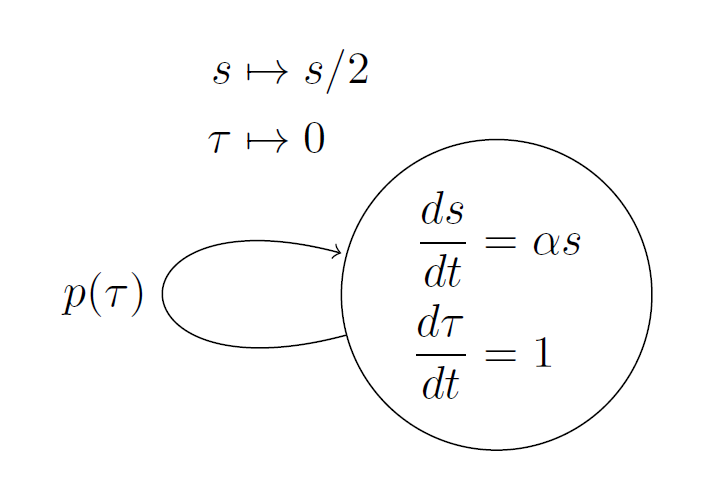
\includegraphics[width=3.83333in,height=\textheight]{./hsys.png}

}

\caption{Growth and cell division representation using automata
notation.}

\end{figure}

Cell size \(s\) at a given experimental time \(t\) can be written as the
combination of sizes in individual cell cycles, that is,
\[\begin{aligned}
    s(t)=\sum_{n=0}^{\infty} s_n(t) P_n(t),
\end{aligned}\] where \[\begin{aligned}
    s_n(t)=&s_{0}\left[\prod_{i=1}^{n} \frac{e^{\alpha\left(t_{i}-t_{i-1}\right)}}{2}\right] e^{\alpha\left(t-t_{n}\right)}\\
    =&\frac{s_0}{2^n} e^{\alpha t}
\end{aligned}\] is the cell size \(s\) at experimental time \(t\) given
cell performed \(n\) divisions. The sequence of experimental times at
which division happens is \(t_i\) with \(t_i-t_{i-1}=\bar{\tau}\). The
cell cycle time after \(n\) divisions is given by \(\tau=t-t_n\).
\[P_n(t)=\begin{cases}
    1,  \text{ if }\quad n\,\bar{\tau} < t \leq (n+1)\bar{\tau}  \\
    0,  \text{ otherwise}
\end{cases}\] dictates the number of cell cycles \(n\) performed by the
cell at time \(t\). Cell size \(s(t)\) is a periodic function in time,
with a period \(\bar{\tau}\) and a repeating dynamics represented by
exponential growth \(s_0e^{\alpha t}\) in the cell cycle interval
\(\tau \in [0,\bar{\tau}]\).

\hypertarget{division-mechanisms-the-timer-the-sizer-and-the-adder}{%
\section{Division mechanisms: the timer, the sizer, and the
adder}\label{division-mechanisms-the-timer-the-sizer-and-the-adder}}

We also can track key features of the cell cycle such as division time
\(\tau_d\), newborn \(s_b\), division \(s_d\), and added size \(s_a\).
The feature \(s_c\) records the newborn cell size of the next division
event. Let \[\mathbf{x}=[s_d,s_a,s_b,s_c,\tau_d, s, n, \tau]\] be the
vector of cell cycle features. At the beginning of the experiment
\(s_b(0)=s_c(0)=s_0\), \(s_a(0)=\tau_d(0)=0\). At the end of the first
cell cycle, the size at division resets to the current cell size
\(s_d \mapsto s\), then we compute the added cell size
\(s_a\mapsto s-s_b\), the newborn cell size becomes half the division
size \(s_b \mapsto s/2,\) the number of cell cycles performed resets to
\(n\mapsto n+1,\) and the cell cycle time resets to zero
\(\tau \mapsto 0.\)

It is important to maintain the order in the resets performed.
Preserving this order of updating features ensures that once a cell
cycle ends, \(s_c\) records the newborn size of the next cell cycle
event. The updated vector of features is
\[\phi(\mathbf{x})=[s,s-s_b,s_c,s/2,\tau,s/2,n+1,0].\] The modified
graph summarizing the cell division dynamics is shown in Fig 2.

\begin{figure}

{\centering 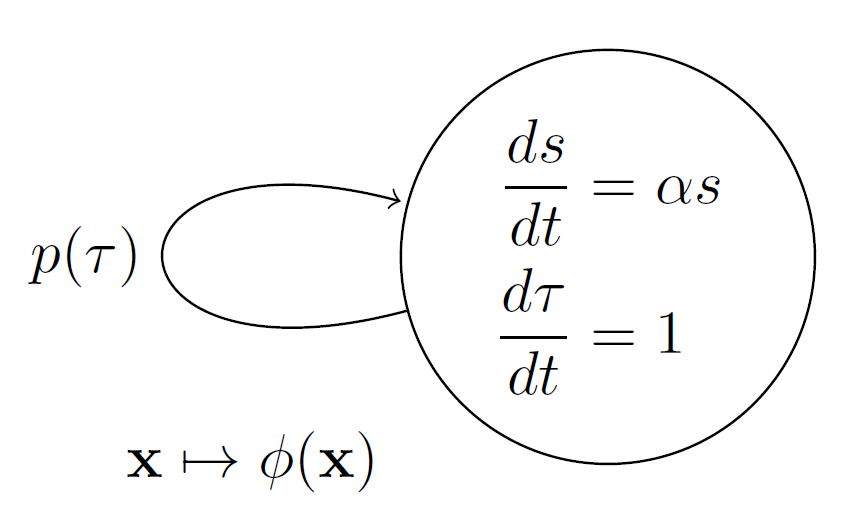
\includegraphics[width=3.83333in,height=\textheight]{./shsm.png}

}

\caption{Growth and cell division representation using automata
notation.}

\end{figure}

The relationships between \(s_b\), \(s_d\), \(s_a\), and \(\tau_d\)
describe the division control mechanism \cite{}. For any cell cycle,
assuming that the cell cycle time \(\tau_d[n]=\bar{\tau}\) is kept fixed
over generations using the division rate
\(p(\tau)=\delta(\tau-\bar{\tau})\), we have
\(s_d=s_b e^{\alpha \bar{\tau}}\) and
\(s_a=s_d-s_b=s_b (e^{\alpha \bar{\tau}}-1)\). This is known as the
\textbf{timer} strategy for cell division. For any cell cycle \(n\) we
see that the size of the newborn cell \(s_b[n]\) is affected by the size
of the newborn cell in the previous generation, i.e.,
\[s_b[n]=\frac{e^{\alpha \bar{\tau}}}{2}s_b[n-1]\]. This recursion can
be rewritten as a function of the number of cell cycles \(n\)
\[s_b[n]= \frac{e^{n \alpha \bar{\tau}}}{2^{n}} s_0.\] Division size at
any cell cycle is given by
\[s_d[n]= \frac{e^{(n+1) \alpha \bar{\tau}}}{2^{n}} s_0.\] Added size
series are
\[s_a[n]= (e^{\alpha \bar{\tau}}-1)\frac{e^{n \alpha \bar{\tau}}}{2^{n}} s_0.\]
These series converges to a non-zero finite value only when
\(\tau_d=\bar{\tau}=\log{2}/\alpha.\) This reduces the size at division
to \(s_d=2 s_b\), and the added size in any cycle to \(s_a=s_b\). This
implies that for any timer strategy, we will find a slope of 2 when we
plot the size at division \(s_d\) vs.~newborn size \(s_b\). Plotting
added vs.~newborn size gives a slope of one.

If we assume the cell divides by the division rate
\(p(s)=\delta(s-\bar{s})\), for any cell cycle \(n>1\) then we have
\[s_d[n]=\bar{s},\, s_b[n]=\bar{s}/2,\, \text{and } \, \tau_d[n]=\log{2}/\alpha.\]
Such division strategy is known as \textbf{sizer}.

An alternative to this division mechanism is considering that the cell
aims to add a fixed amount of size at any cell cycle. Let the division
rate be \(p(s)=\delta(s-s_b-\Delta)\), then the size at birth at any
cell cycle \(n\) is \[\begin{aligned}
    s_b[n]=&\frac{s_b[n-1]+\Delta}{2}\\
    =&\frac{s_0+(2^n-1)\Delta}{2^n}
\end{aligned}\] where \[\lim_{n\to \infty}s_b[n]=\Delta.\] Such division
strategy is know as \textbf{adder}. Size at division for the \(n\) cell
cycle is given by \[
s_d[n]=2^{-n}(s_0 -\Delta)+2 \Delta, \, \lim_{n\to \infty}s_d[n]=2 \Delta.
\]

Division time at any cell cycle is given by \[\begin{aligned}
    \tau_d[n]=&\frac{1}{\alpha}\log \frac{s_d[n]}{s_b[n]}\\
    =&\frac{1}{\alpha}\log\left({2+\frac{\Delta-s_0}{s_0+(2^n-1)\Delta}}\right), 
\end{aligned}\] where
\[\lim_{n\to \infty}\tau_d[n]=\frac{\log 2}{\alpha}.\] All division
strategies can be summarize when assuming a division rate
\(\delta(s-b\,s_b-a)\). Size at birth in any cell cycle is given by \[
s_b[n]=\frac{b^n(a+(b-2)s_0)-2^n\,a}{2^n(b-2)}.
\] Note the special cases \(b=1\), \(a=\Delta\) as adder and \(b=0\) as
sizer. The size at division is given by \[
s_d[n]=a+\frac{b^{n+1}(a+(b-2)s_0)-2^nba}{2^n(b-2)}.
\] Cell cycle time is given by \[
\tau[n]=\frac{1}{\alpha}\log \left[b-\frac{2^n a(b-2)}{2^n a-b^n(a+(b-2) s_0)}\right].
\]

\bookmarksetup{startatroot}

\hypertarget{summary}{%
\chapter{Summary}\label{summary}}

In summary, this book has no content whatsoever.

\begin{Shaded}
\begin{Highlighting}[]
\DecValTok{1} \SpecialCharTok{+} \DecValTok{1}
\end{Highlighting}
\end{Shaded}

\begin{verbatim}
[1] 2
\end{verbatim}

\bookmarksetup{startatroot}

\hypertarget{references}{%
\chapter*{References}\label{references}}
\addcontentsline{toc}{chapter}{References}

\markboth{References}{References}

\hypertarget{refs}{}
\begin{CSLReferences}{0}{0}
\end{CSLReferences}



\end{document}
